\documentclass[12pt, letterpaper]{article}
\usepackage{graphicx}
\title{Fast Trajectory Replanning Report}
\author{Xinyu Meng xm73 Qichao Lin ql180}
\date{Feb 21 2023}
\begin{document}
\maketitle
\section{Part 1}
\subsection{a}

Explain in your report why the first move of the agent for the example search problem from Figure 8 is to the east rather than the north given that the agent does not know initially which cells are blocked.

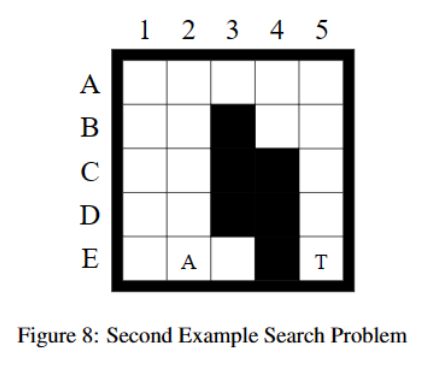
\includegraphics{part1a.png} 

In the above example, based on the A* algorithm, the north node has g = 1, h = 3+1 = 4, therefore f = g+h = 5.

The east node has g = 1, h = 2, f = 3. The first iteration of A* will make the agent go straight to the right as it will pick the lowest f in the open list. Therefore the execution will follow what A* initially planned to move to the east. 

\subsection{b}

This project argues that the agent is guaranteed to reach the target if it is not separated from it by blocked cells. Give a convincing argument that the agent in finite gridworlds indeed either reaches the target or discovers that this is impossible in finite time. Prove that the number of moves of the agent until it reaches the target or discovers that this is impossible is bounded from above by the number of unblocked cells squared.


To prove that repeated A* cannot repeat forever in a grid where there is a path to the goal from the initial state, we can use the fact that A* is guaranteed to find the shortest path to the goal if one exists. Therefore, if the agent is moving in an infinite loop, it means that there is no shorter path to the goal than the one it is currently following. However, this contradicts the assumption that there is a path to the goal from the initial state, since if there is a path, the A* will in fact return the correct path to the goal. If the A* algorithm reaches a dead end, where there are no more unexplored cells that are reachable from the current cell, it will backtrack to the previous cell and continue exploring from there. However, since the A* algorithm evaluates cells in order of increasing cost, it will eventually evaluate the cell that leads to a path to the target cell, and it will terminate.Also, as the A* has a mechanism to record the obstacles explored by the executed path, A* will return null if there is no possible path based on the explored map, which will stops the execution if there is not possible path exist. 

Moreover, in the worst case, the agent will execute all the unblocked nodes before get stuck. Then, the agent will keep planning and execute all the unblocked nodes again until it reaches a block. Under such scenario, the agent can only start an A* from a unblocked node once and therefore the total number of executions of the agent in the worst scenario is bounded by the square of the number of the unblocked nodes.

\section{Part 2 - The Effect of Ties}

path found by repeated A* with normal priority

execution time: 1.068s

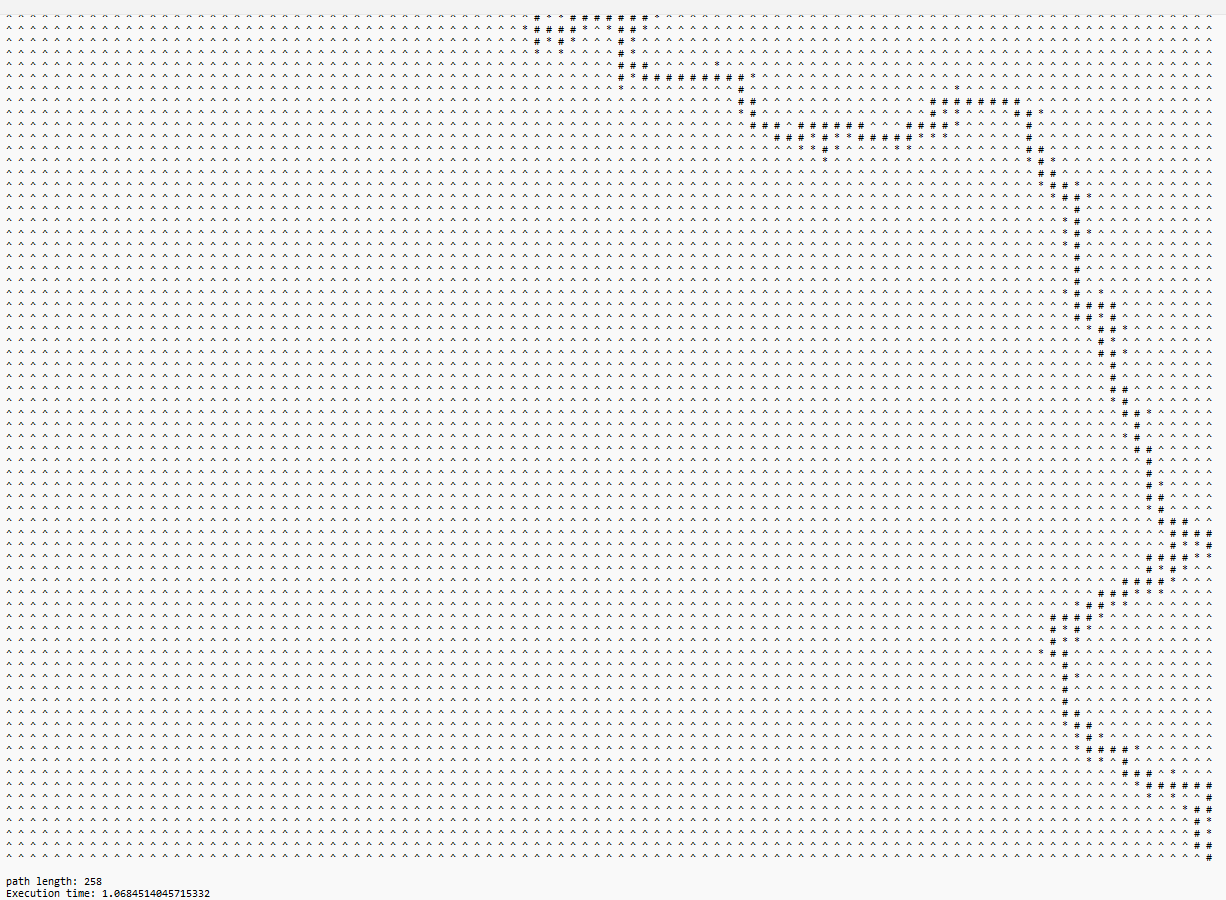
\includegraphics[width=\textwidth,height=\textheight]{part2a.png} 

path found by repeated A* with priority = 203*f - g
203 means this constant is greater than any g value

execution time: 0.723s

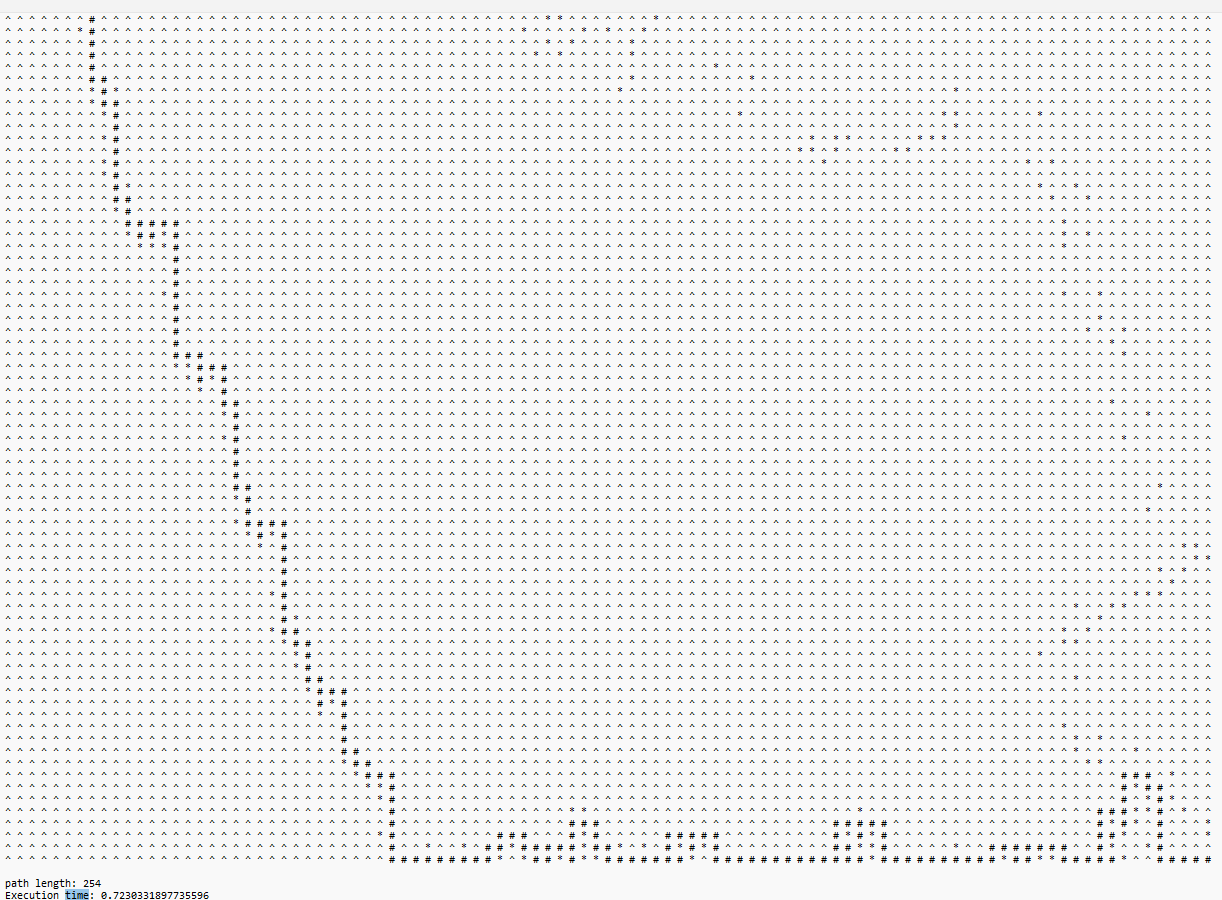
\includegraphics[width=\textwidth,height=\textheight]{part2b.png}

Since we use priority = cf - g where f = g+h

priority = c(g+h) - g = cg + ch - g = (c-1)g + ch

g has higher weigh in the priority, when tie-breaking in favor of cells with smaller g-values, the algorithm tends to prioritize expanding cells that are closer to the start state, which are likely to be part of a shorter path to the goal. On the other hand, when tie-breaking in favor of cells with larger g-values, the algorithm tends to prioritize expanding cells that are further from the start state, which may be part of longer paths to the goal. 

\section{Part3}

Forward A* execution time: 1.1978s

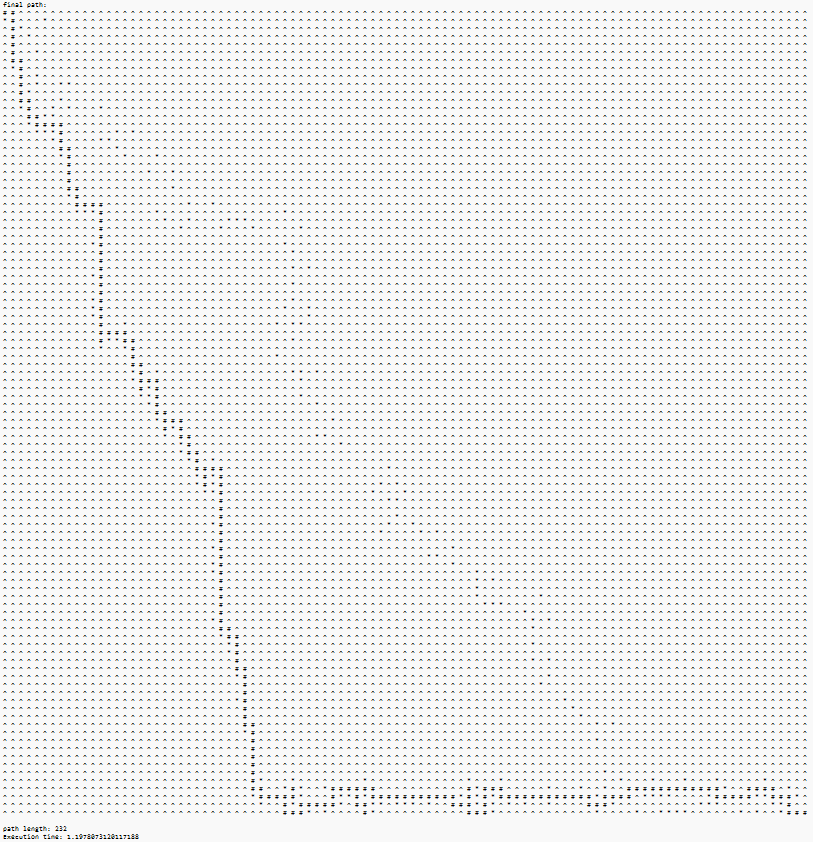
\includegraphics[width=\textwidth,height=\textheight]{part3a.png}

Backward A* execution time: 0.7894s

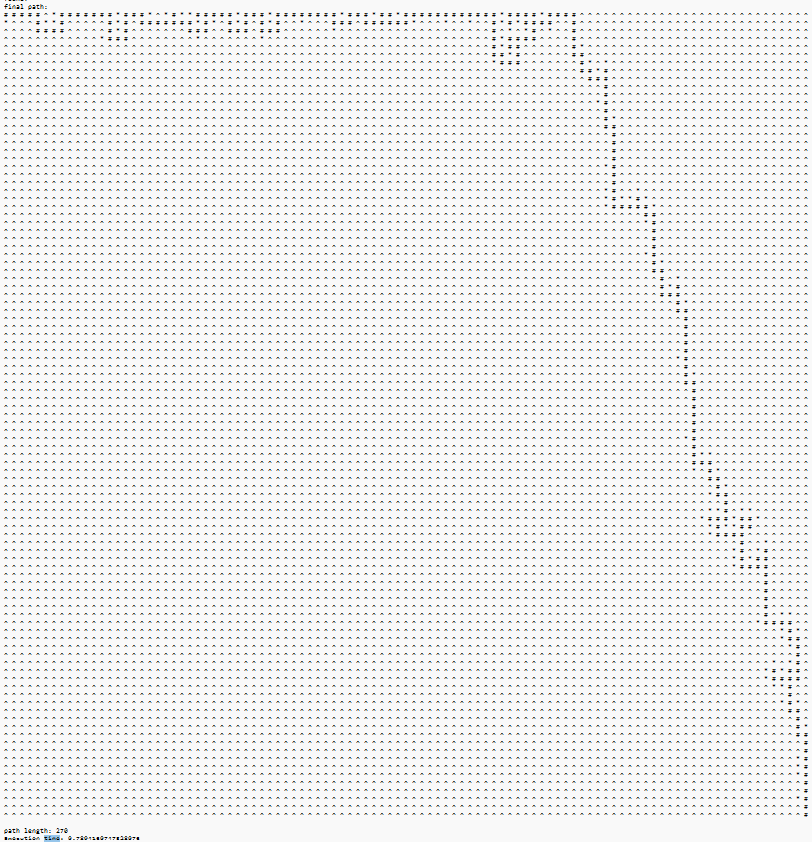
\includegraphics[width=\textwidth,height=\textheight]{part3b.png}

In most situations Repeated Backward A* performs better than Repeated Forward A*, in terms of both number of expanded cells and runtime. This is because Repeated Backward A* algorithm may be able to more quickly identify the shortest path to the goal by first exploring the cells closer to the goal state, which are more likely to be part of the shortest path. In contrast, Repeated Forward A* may waste time exploring parts of the grid that are not relevant to the shortest path. But in some mazes, Forward A* may be faster than Backward A* due to the setting of obstacles.

\section{Part4}

Consistent heuristic meets the condition that the estimated cost of reaching a goal from a given node is always less than or equal to the cost of reaching any successor node, plus the estimated cost of reaching the goal from that successor node. Therefore, h(n) <= c(n, a, n') + h(n'). 

Consider two adjacent nodes, n and n' assume that the agent can only move in the four main compass directions (north, south, east, west). Then the cost of moving from n to n' is always 1, regardless of the action taken. h(n) = abs(n.x-g.x) + abs(n.y-g.y) and h(n') = abs(n'.x-g.x) + abs(n'.y-g.y)

by triangle inequality:

h(n) = abs(n.x-n'.x+n'.x-g.x) + abs(n.y-n'.y+n'.y-g.y) and h(n') = abs(n'.x-n.x+n.x-g.x) + abs(n'.y-n.y+n.y-g.y)

after simplify, we get

h(n) = h(n')+1+abs(n.x-n'.x)+abs(n.y-n'.y)-2abs(n'.x-n.x)-2abs(n'.y-n.y)

since the agent can only move in the four main compass directions, abs(n.x-n'.x) and abs(n.y-n'.y) can only be 0 or 1. Therefore, we can simplify the inequality to:

h(n) <= h(n') + 1, which proves that the Manhattan distance heuristic is consistent in gridworlds where the agent can only move in the four main compass directions.

Adaptive A* leaves initially consistent h-values consistent even if action costs can increase.

Suppose we have a consistent heuristic function h(s) that is initially admissible for a gridworld with action costs that may increase. Let hnew(s) be the new heuristic function obtained by updating the estimated costs of reaching the goal from each node s, based on the actual costs of reaching s from the start node. If the h-values consistent, h(n) <= c(n, n') + h(n'), where c(n, n') is the cost of moving from n to n'.

In Adaptive A*, the heuristic values h(n) are updated based on the actual costs of the paths found during the search, rather than being fixed at the beginning of the search. Specifically, when a new path is found that is cheaper than the previously known path to a node n, the heuristic value h(n) is updated to the actual cost of the new path plus the estimated cost of reaching the goal from the end of the new path. This new value of h(n) is guaranteed to be admissible, as it is based on the actual cost of the path found. Suppose that we have two nodes n and n' such that h(n) > c(n, n') + h(n'). If the cost of moving from n to n' increases, the actual cost of the path from the start node to n' may increase as well. However, when Adaptive A* considers the node n again, it will find a cheaper path to n' that takes into account the increased action costs. Specifically, the actual cost of the path from the start node to n' will be updated, and the heuristic value h(n) will be updated to the actual cost of the new path plus the estimated cost of reaching the goal from n'. Because the estimated cost of reaching the goal from n' is fixed and the new path has a higher actual cost, the new value of h(n) will still be less than c(n, n') + h(n'). Therefore, the consistency of the heuristic function is maintained even if the action costs increase. Therefore, the Adaptive A* will keeps the h values consistent.

\section{Part5}

Forward A* tie-breaking execution time: 0.7832608222961426

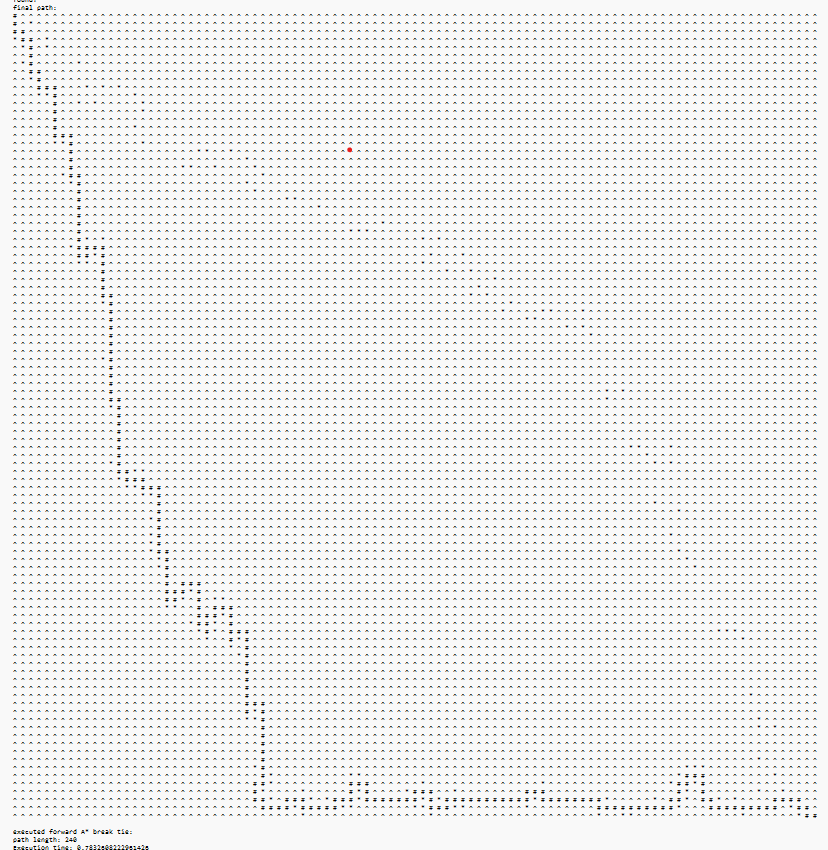
\includegraphics[width=\textwidth,height=\textheight]{part5a.png}

Adaptive A* tie-breaking execution time: 0.7628557682037354

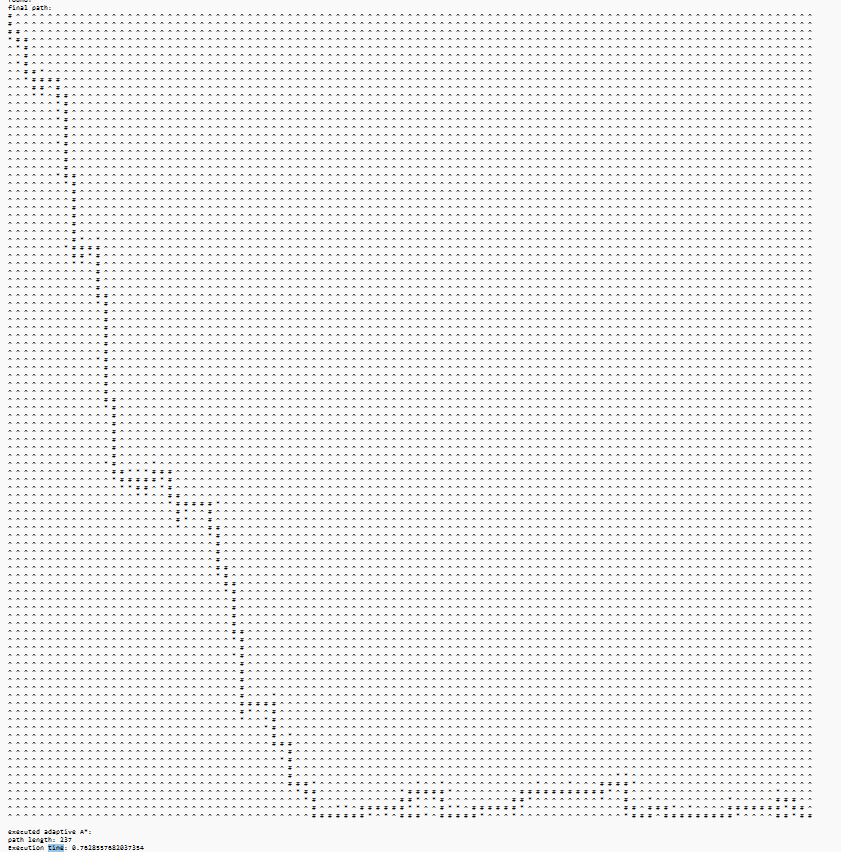
\includegraphics[width=\textwidth,height=\textheight]{part5b.png}

Repeated Adaptive A* perform better than Repeated Forward A* in some cases because it has access to more information about the search state and can adapt its heuristic values more efficiently. However, the improvement in performance may not be significant in all cases, and the specific characteristics of each maze may affect the runtime differently for each algorithm.

Also, the Repeated Forward A* perform better in some other mazes. This is because the Repeated Forward A* seems gets more advantages by using the tie-breaking approach over Adaptive A*. The overall direction for the final paths for each A* is similar while they still vary in details. 

\section{Part6}

On the problem above "Forward vs Backward" we can perform a statistical hypothesis to verify if the repeated Forward A* and repeated Backward A* have a systematic difference in their runtime. 

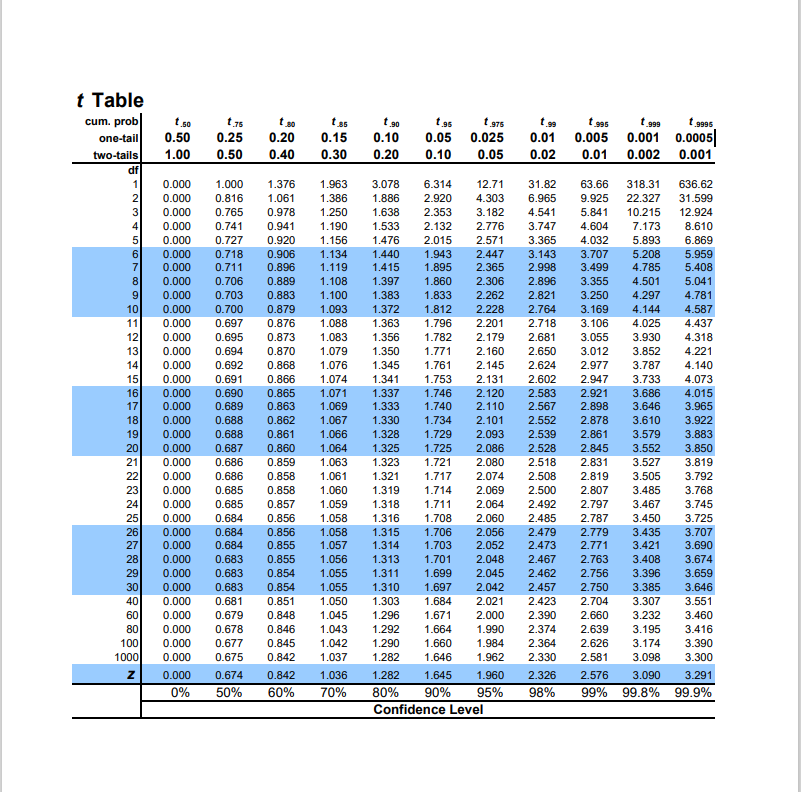
\includegraphics[width=\textwidth,height=\textheight]{part6a_t_table.png}


By using t-test

t = (avg1 - avg2) / (sqrt((s1**2/n1) + (s2**2/n2)))

Where avg1 is the average running time of Repeated Forward A*, avg2 is the average running time of Repeated Backward A*, s1 is the standard deviation of Repeated Forward A* running time, s2 is the standard deviation of Repeated Backward A* running time, n1 is the number of data of Forward A*, n2 is the number of data of Repeated Backward A*.

Get the degrees of freedom using: df = n1 + n2 - 2

Finding the critical t-value in the t-table using the degrees of freedom and the desired level of significance.

Compare the calculated t-value with the critical t-value. If the calculated t-value is greater than the critical t-value, we reject the null hypothesis which means there is a systematic difference in the runtime of the Repeated Forward A* and Repeated Backward A*. If the calculated t-value is less than the critical t-value, we fail to reject the null hypothesis.

\end{document}